\chapter{Simulated Environment}\label{ch:simulated.environment}

As drones are expensive and fragile machines with a very limited autonomy, it is common practice to carry out the first tests on a simulator. Before starting any manipulation with drones, a simulator was therefore chosen and two simulated indoor environments were created.

This chapter reviews the main existing simulators, the characteristics of the chosen one and describes the simulated environments created.

\section{Simulator}

A simulator is a tool for reproducing real actions in a virtual environment.

When working with drones, and robots in general, it is essential to carry out preliminary tests so as not to damage the machine or endanger the working environment. In the case of drones, the very limited battery (just a few minutes for MAVs) is an additional problem that can limit real-life testing; hence the importance of a simulator.

For the tests to be realistic, the simulator must be able to model the real world and the drone as faithfully as possible: the forces applied, the possible turbulence, the wind, the movements that are not always precise, but also the brightness of the rooms, the shadows, the blurred images due to the movements, etc.

Although there are many physical simulators, two of them stand out in the drone field: Gazebo and Unreal Engine 4.

\subsection{Gazebo}

Gazebo \cite{gazebo2021website} is an open-source simulator developed by the Open Robotics \cite{openrobotics2021website} company. As mentioned on the official website, \enquote{\textit{Gazebo offers the ability to accurately and efficiently simulate populations of robots in complex indoor and outdoor environments}} \cite{gazebo2021website}.

With its numerous plugins, developed largely by the community, and compatible with the Robot Operating System (ROS) \cite{ros2021website}, also developed by Open Robotics, Gazebo is a very popular simulator for robots. It is lightweight and available on all platforms.

Gazebo was not created to simulate drones exclusively. It is therefore necessary to manually add and configure all the resources needed. The documentation is also not specifically oriented to the use of drones, making it sometimes difficult to get familiar with the tool.

\subsection{Unreal Engine 4}

Unreal Engine \cite{unrealengine2021website} (version 4) is a proprietary game engine developed by the Epic Games \cite{epicgames2021website} company. Initially created for video games, Unreal Engine has now become very popular for a wide range of applications: architecture, 3D modeling, animation and film making, simulations, etc. Its realism and the quality of its rendering have made it one of the most popular game engines on the market.

The disadvantages of Unreal Engine are that it is quite heavy (a high-performance hardware configuration is necessary) and, despite a compatibility announced on all platforms, it is usable correctly only on the Windows operating system.

Being initially a game engine, Unreal Engine is not designed to perform robot simulations. However, being extremely rich in the possibilities it offers, it is possible to set up simulated environments and robots via additional plugins.

\subsubsection{AirSim}

AirSim \cite{shah2018airsim} is an open-source plugin, developed by the Microsoft company, for Unreal Engine allowing a realistic simulation of cars and drones. It adds all the necessary functionalities to have a simulated environment taking advantage of the very high realism of the game engine.

The great advantage of AirSim is that it has been developed with the aim of simulating drones, and more specifically via Artificial Intelligence systems. An API, developed in Python, is available with all the necessary functionalities to easily set up autonomous and intelligent systems (\eg{} easy image collection and annotation). A whole series of sensors and images are available and can be used directly (LIDAR, segmented images, depth map), making the constitution of data sets relatively fast and easy.

The plugin has been designed to be as faithful as possible to the real world. Combined with the high level of realism of the Unreal Engine, it is possible to obtain simulations that are extremely faithful to the real behavior of a drone in a real environment.

\subsection{Comparison}

The two simulators, Gazebo and Unreal Engine with AirSim, both offer interesting possibilities for drone simulation. Although still less mature than Gazebo, AirSim is gradually gaining popularity so that it is widely used in the drone field.

Both simulators are compatible with all platforms, although AirSim (with Unreal Engine) is only usable easily (configuration and running) on Windows. However, the drone-simulated oriented aspect and the ready-to-use Python interface of the latter has been preferred, and therefore used, for this project.

\begin{note}
    All the precise technical characteristics of the machine used to run the simulator as well as the different versions of the programs and languages used in this work are described in Appendix \ref{ch:technical.specifications}.
\end{note}

\section{Environments}

The next step is to create simulated environments. It is important that these environments are as realistic as possible and faithful to the real world. Indeed, working mainly with images from the drone, the more realistic the environment, the closer the images will be to real images and the better the algorithms can be adapted to real conditions.

The real reference environment being the main building of the Montefiore Institute at the University of Liège, the objective is to create simulated environments composed of corridors, turns and other characteristic elements (doors, decorations, lamps, etc.). In order to test the efficiency and generalization of the algorithms, it would be ideal to work with at least two different environments.

\subsection{Resources already available}

A wide range of assets (3D modeled objects but also complete ready-made environments) are available via the Unreal Engine Marketplace. Unfortunately, the majority of them are not free. The few free resources do not correspond to the desired environment characteristics.

Apart from the Unreal Engine Marketplace, there are few ready-to-use indoor environments for Unreal Engine available for free. Another interesting resource is the PEDRA project \cite{anwar2020autonomous}, which offers a series of simulated indoor environments that match the desired environment characteristics. Unfortunately, these are not editable (either the simulation parameters or the environment itself and its components) and were created with an old version of AirSim. They are therefore difficult to use for this project.

\subsection{Handcrafted resources}

As no resources matching the characteristics of the Montefiore Institute were available, two open-source simulated environments on Unreal Engine has been designed for this project (see Section \ref{sec:01.resources} for download links).

The two environments created are called \enquote{Indoor Corridor} and \enquote{Indoor Staircase}. All the 3D objects used come from free resources available on the Unreal Engine Marketplace.

\subsubsection{Indoor Corridor}

Indoor Corridor is a simulated environment composed of 5 corridors, 4 turns and 2 crossroads. The extreme corridors have doors and the whole environment is composed of various decorations (plants, frames, chairs, armchairs). Lamps are displayed on each wall. Their intensity has been adjusted so that their effect on the environment is realistic: the corridors are fairly well lit, but some areas, such as the corners, are a little less so. The floor has a wooden floor texture to be faithful to the Montefiore Institute.

A series of images illustrating the main elements of the environment is shown in Figure \ref{fig:03.indoor.corridor.images}.

\begin{figure}[H]
    \centering
    \begin{subfigure}[b]{0.48\textwidth}
        \centering
        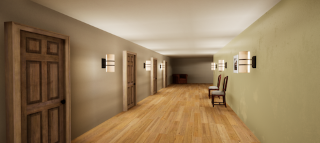
\includegraphics[width=\textwidth]{resources/png/03/indoor-corridor/1.png}
        \vspace{0.25em}
    \end{subfigure}
    \hfill
    \begin{subfigure}[b]{0.48\textwidth}
        \centering
        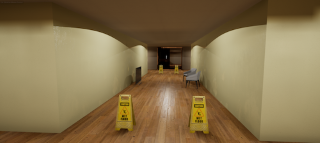
\includegraphics[width=\textwidth]{resources/png/03/indoor-corridor/2.png}
        \vspace{0.25em}
    \end{subfigure}
    \begin{subfigure}[b]{0.48\textwidth}
        \centering
        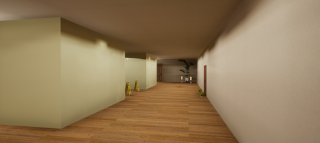
\includegraphics[width=\textwidth]{resources/png/03/indoor-corridor/3.png}
    \end{subfigure}
    \hfill
    \begin{subfigure}[b]{0.48\textwidth}
        \centering
        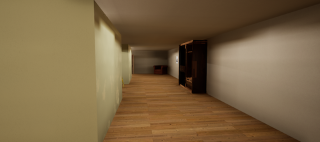
\includegraphics[width=\textwidth]{resources/png/03/indoor-corridor/4.png}
    \end{subfigure}
    \caption{Images of the Indoor Corridor simulated environment.}
    \label{fig:03.indoor.corridor.images}
\end{figure}

A video illustrating the environment in more detail is available via the following link: \url{https://youtu.be/cz1zRka21UY}.

\subsubsection{Indoor Staircase}

Indoor Staircase is an environment strongly inspired by Indoor Corridor. The basic shape is identical, but all the textures and decorative objects are different. The central corridor has also been replaced by a staircase leading to a floor consisting of a single corridor.

This environment will be used to test the generalization of the algorithms and to try to teach the drone to autonomously fly over staircases.

A series of images illustrating the main elements of the environment is shown in Figure \ref{fig:03.indoor.staircase.images}.

\begin{figure}[H]
    \centering
    \begin{subfigure}[b]{0.48\textwidth}
        \centering
        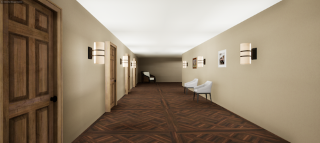
\includegraphics[width=\textwidth]{resources/png/03/indoor-staircase/1.png}
        \vspace{0.25em}
    \end{subfigure}
    \hfill
    \begin{subfigure}[b]{0.48\textwidth}
        \centering
        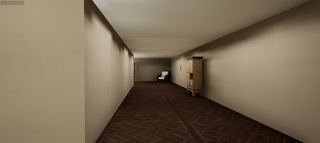
\includegraphics[width=\textwidth]{resources/png/03/indoor-staircase/2.png}
        \vspace{0.25em}
    \end{subfigure}
    \begin{subfigure}[b]{0.48\textwidth}
        \centering
        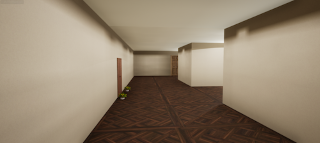
\includegraphics[width=\textwidth]{resources/png/03/indoor-staircase/3.png}
    \end{subfigure}
    \hfill
    \begin{subfigure}[b]{0.48\textwidth}
        \centering
        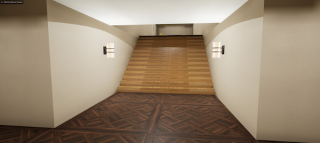
\includegraphics[width=\textwidth]{resources/png/03/indoor-staircase/4.png}
    \end{subfigure}
    \caption{Images of the Indoor Staircase simulated environment.}
    \label{fig:03.indoor.staircase.images}
\end{figure}

A video illustrating the environment in more detail is available via the following link: \url{https://youtu.be/muzKT-dCab4}.

\subsubsection{Aerial views}

In order to give a better idea of the structures of each of the simulated environments, aerial views are presented in Figure \ref{fig:03.aerial.views}.

\begin{figure}[H]
    \centering
    \begin{subfigure}[b]{0.48\textwidth}
        \centering
        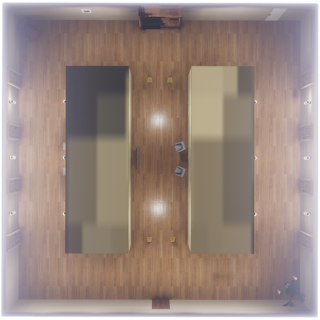
\includegraphics[width=\textwidth]{resources/png/03/indoor-corridor/aerial.png}
        \caption{Indoor Corridor}
    \end{subfigure}
    \hfill
    \begin{subfigure}[b]{0.48\textwidth}
        \centering
        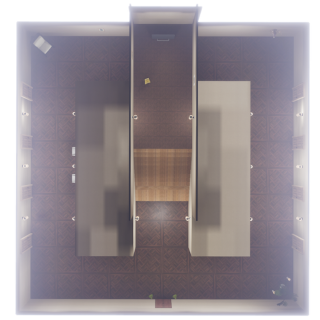
\includegraphics[width=\textwidth]{resources/png/03/indoor-staircase/aerial.png}
        \caption{Indoor Staircase}
    \end{subfigure}
    \caption{Aerial views of the simulated environments.}
    \label{fig:03.aerial.views}
\end{figure}
